%\newpage
\section{Tieftöner-Messungen} \label{sec:5.3}
\subsection{Einleitung} \label{subsec:5.3.1}
Tieftöner sind, wie der Name bereits andeutet, für den unteren Frequenzbereich gedacht und konzipiert.
In diesem Projekt werden Tieftöner-Lautsprecher an zwei verschiedenen Positionen verwendet:
\begin{itemize}
	\item Im Subwoofer und 
	\item in der Satellitenbox
\end{itemize}
Es ist so angedacht, dass der Subwoofer (Mono) nur die sehr niedrigen Frequenzen übernimmt.
Er ist bis ca. 200 Hz aktiv.\\
In den Satellitenboxen ist jeweils ein kleinerer Tieftöner verbaut, um den Übergang zwischen sehr tiefen und hohen Frequenzen zu bilden.
Diese zwei Lautsprecher (Stereo) arbeiten ebenfalls bei niedrigen als auch bei mittleren bis hohen Frequenzen.
Die Grenze des Satelliten-Tieftöners liegt bei ca. 5 kHz.

\subsection{Ziele} \label{subsec:5.3.2}
Der Lautsprecher für die Subwoofer-Box muss größer und leistungsfähiger sein, um die richtig tiefen Frequenzen möglichst gut abzustrahlen.
Da er nur bis ca. 200 Hz aktiv ist, sollte der Frequenzgang genau in diesem Bereich einen hohen Schalldruckpegel aufweisen.
Der Rest des Frequenzganges ist nicht so wichtig, da der Lautsprecher auch nicht in einem höheren Bereich verwendet wird. \\
Bei den Satelliten-Lautsprechern ist der ganz tiefe Frequenzbereich nicht so ausschlaggebend.
Wichtiger ist dafür eine niedrige Welligkeit bis 5 kHz, um den mittleren Frequenzbereich gut abstrahlen zu können.\\ \\
%Welligkeit könnte man vielleicht auch erklären als Grundlage -- @Bointii
Der Messvorgang und -aufbau wurde bereits im Kapitel \ref{sec:5.2} erläutert.
Nach diesem Prinzip wird bei fast allen Messungen vorgegangen.

\newpage
\subsection{Subwoofer} \label{subsec:5.3.3}
Bereits zu Beginn der Diplomarbeit wurde ein großer Tieftöner eingekauft.\\
Dieser wurde in verschiedenen Volumina gemessen.\\
Außerdem wurden Vergleichsmessungen mit einem zweiten Tieftöner durchgeführt.
\begin{figure} [H]
	\centering
	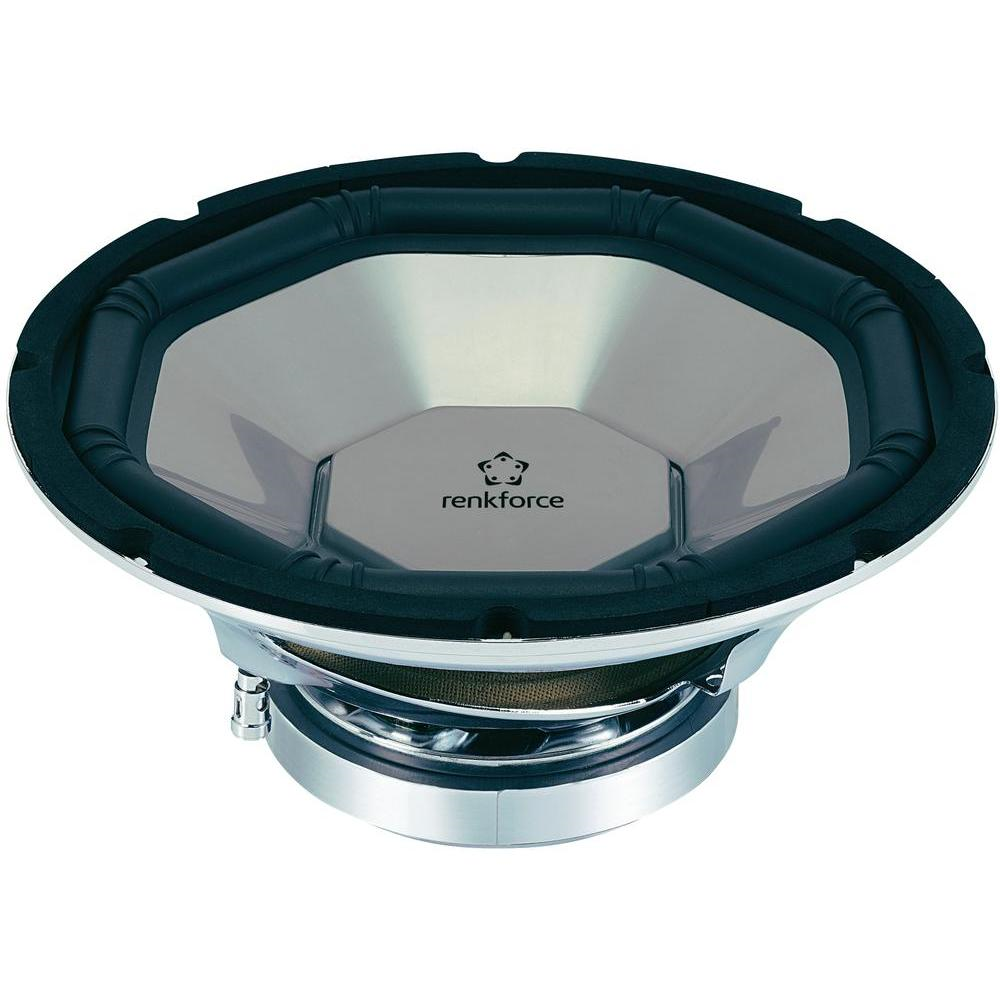
\includegraphics[width=0.5\textwidth]{img/LSMessung/TT/renkforce_B12123.png}
	\caption[\enquote{Renkforce B12123}]{\enquote{Renkforce B12123}\footnotemark}
	\label{fig:5.3.3.1}
\end{figure}
\footnotetext{https://www.conrad.at/de/auto-subwoofer-chassis-300-mm-500-w-renkforce-4-370335.html}
Dieser Lautsprecher wurde ausgewählt, weil er einen vergleichsweise hohen Schalldruckpegel bei tiefen Frequenzen aufweist.
Kurze Spezifikationen des Subwoofers sind:
\begin{itemize}
	\item Maximale Belastbarkeit 500 W
	\item Durchmesser 30 cm
	\item Schalldruck 93 dB
	\item Impedanz 4 $\Omega$
\end{itemize}
Da man eine Box einfacher verkleinern kann als vergrößern, wurde eine Box mit einem Volumen von 149 l für die Messungen verwendet.
Die Box wurde aus Holz gefertigt und mit Silikon abgeschlossen, um mögliche Luftlöcher zu schließen.
Als Vergleichslautsprecher wurde ein \enquote{Visaton WPC30} gemessen.

\newpage
Diese Messungen wurden zu Beginn der Diplomarbeit durchgeführt und daher sind die Ergebnisse so aufgenommen, dass die Einstellungen der Software sichtbar sind.\\ % Ideale Messung beschreiben?
Die zwei Subwoofer wurden einmal mit und einmal ohne Wolle in der Box gemessen. 
\begin{figure} [H]
	\centering
	\subfloat{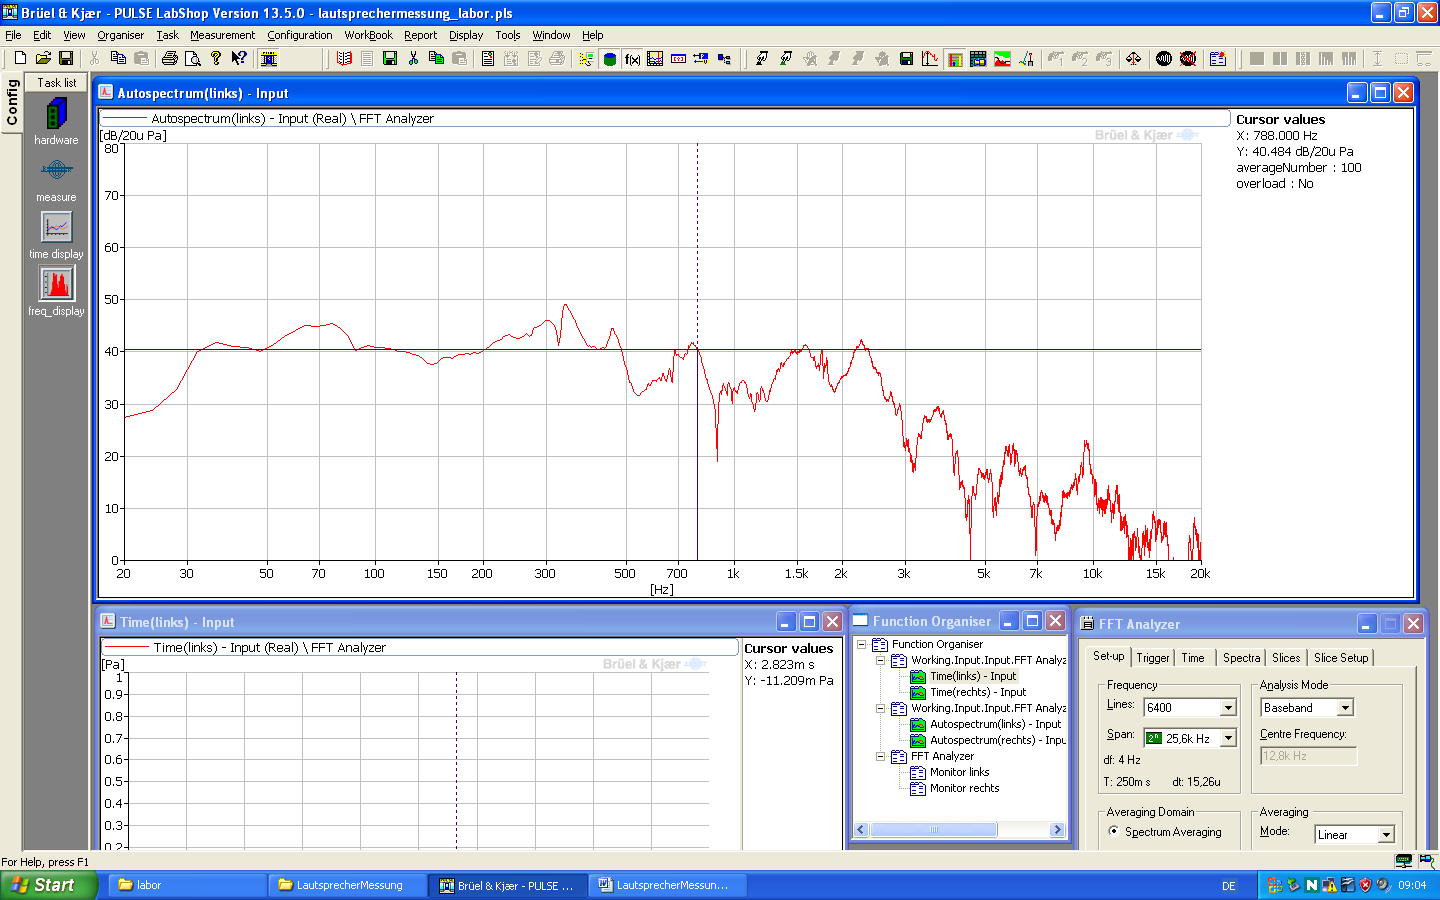
\includegraphics[width=0.75\textwidth]{img/LSMessung/TT/RenkforceOhneWolleMitSilikon.png}}\quad
	\subfloat{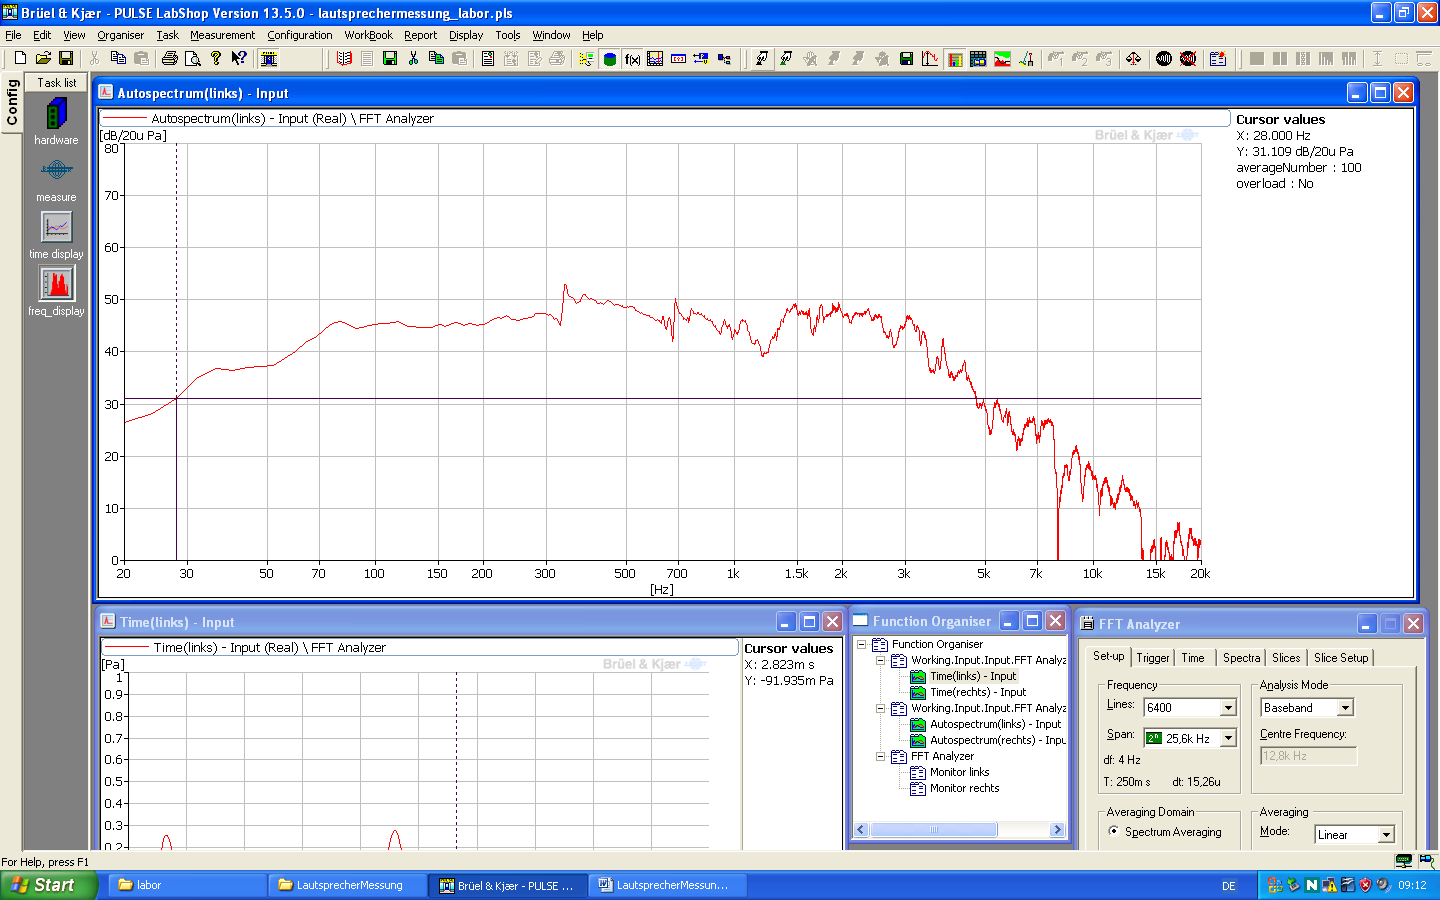
\includegraphics[width=0.75\textwidth]{img/LSMessung/TT/VisatonMitSilikonOhneWolle.png}}
	\caption{Subwoofer-Messung ohne Wolle\\ \enquote{Renkforce} (oben) und \enquote{Visaton} (unten)}
	\label{fig:5.3.3.2}
\end{figure}
Bei diesem Vergleich ist sichtbar, dass der Frequenzgang des \enquote{Visaton}-Tieftöners allgemein \enquote{gerader} ist und weniger Welligkeit aufweist.
Wenn man allerdings nur auf die tiefen Frequenzen achtet, die auch verwendet werden (<200 Hz), ist festzustellen, dass der Schalldruckpegel des \enquote{Renkforce} einen höheren Wert aufweist und daher zu bevorzugen ist.\newpage
Eine weitere Messung mit Wolle in der Box wurde deshalb durchgeführt, weil beide Frequenzgänge bei ca. 300 Hz einen Unregelmäßigkeit aufzeigen.
Die Auswirkungen auf die Lautsprecher sind folgende:
\begin{figure} [H]
	\centering
	\subfloat{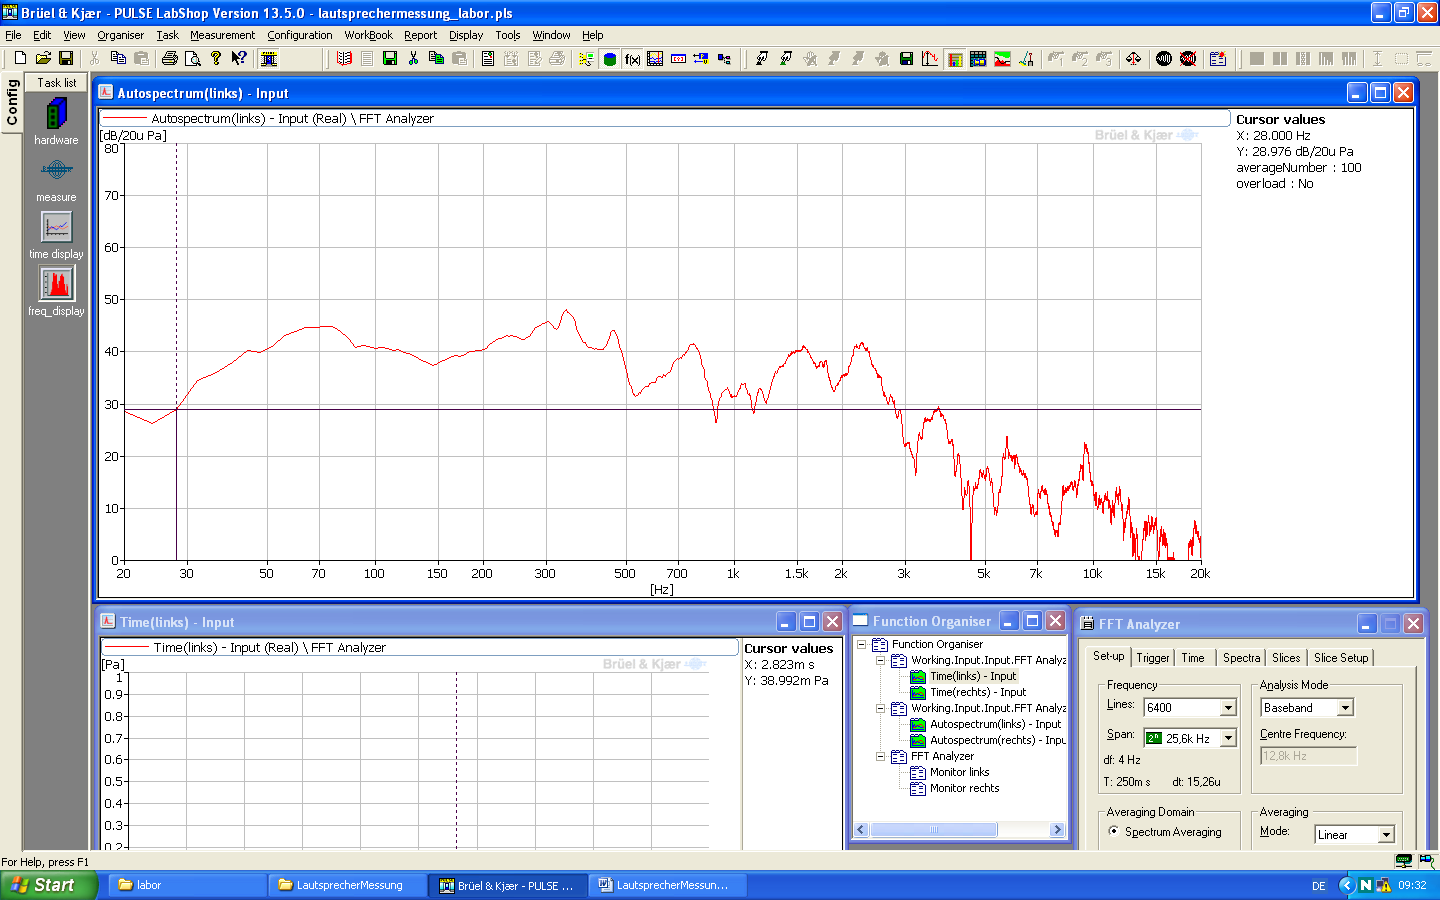
\includegraphics[width=0.75\textwidth]{img/LSMessung/TT/RenkforceMitWolleMitSilikon.png}}\quad
	\subfloat{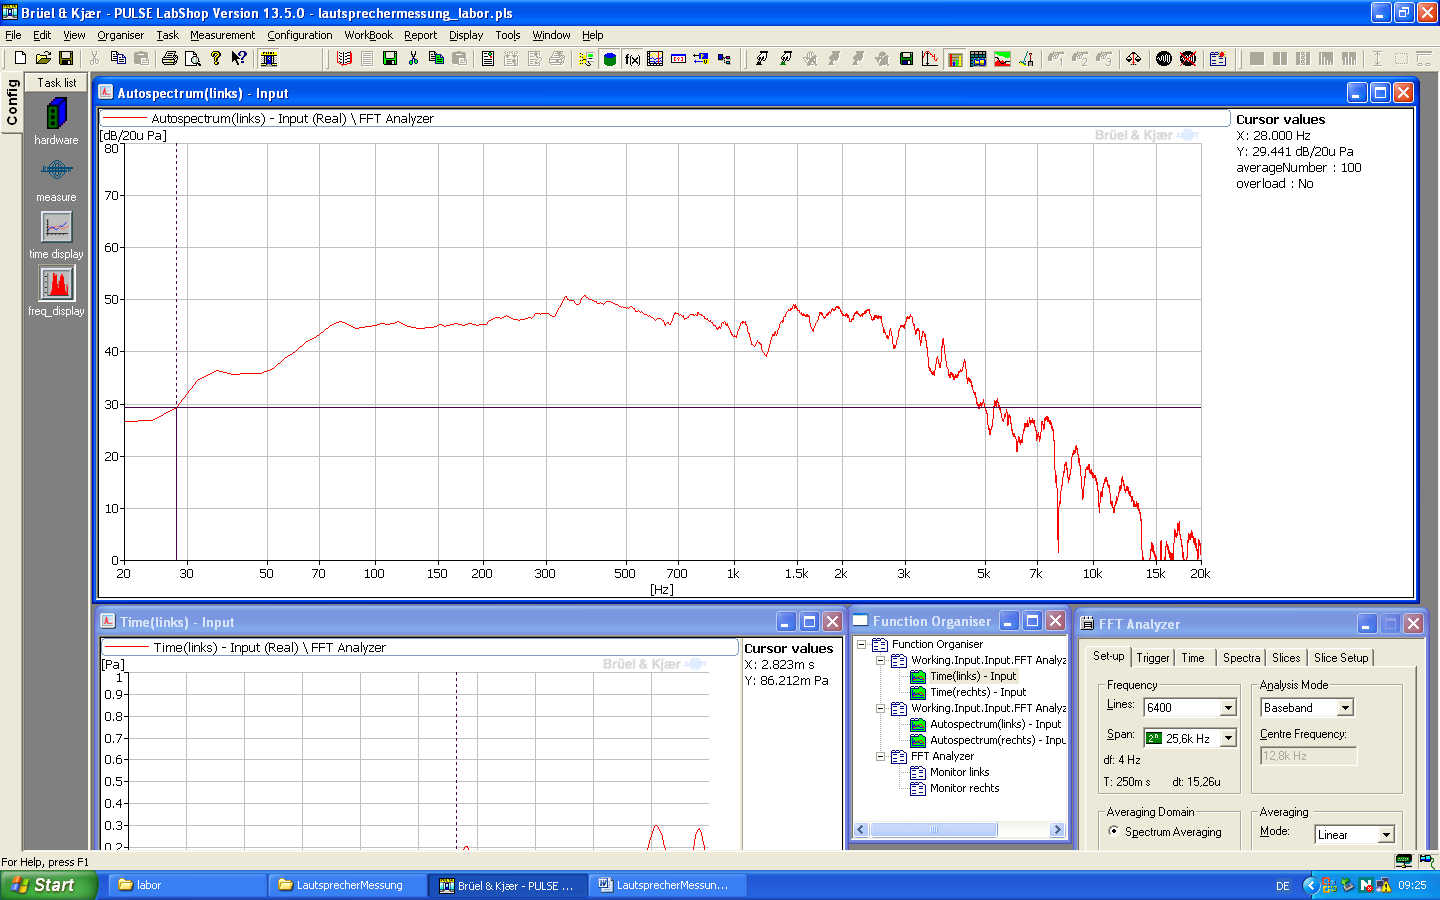
\includegraphics[width=0.75\textwidth]{img/LSMessung/TT/VisatonMitSilikonMitWolle.png}}
	\caption{Subwoofer-Messung mit Wolle\\ \enquote{Renkforce} (oben) und \enquote{Visaton} (unten)}
	\label{fig:5.3.3.3}
\end{figure}
Beide Frequenzgänge wurden durch das Hinzufügen von Wolle etwas \enquote{glatter}, also haben weniger Welligkeit.
Die Wolle kann z.B. stehende Wellen in der Box verhindern und verbessert so deshalb die Eigenschaften der gesamten Box.\\ \\	%Es wirkt wie eine Vergrößerung des Volumens - hat Wagn einmal gsagt
Der Lautsprecher \enquote{Renkforce} weist insgesamt bei tieferen Frequenzen einen höheren Schalldruckpegel auf und wurde auch deshalb von uns für dieses Projekt ausgewählt.


\subsection{Satelliten-Tieftöner} \label{5.3.4}
Als Satelliten-Tieftöner kommen mehrere Lautsprecher in Frage, die vom Betreuer zu Verfügung gestellt wurden.
Die Lautsprecher-Chassis haben einen ähnlichen Durchmesser.
Dadurch können sie in einem Gehäuse (à 13,72 Liter) mit wechselbarer Frontplatte gemessen werden.
Um möglicherweise bessere Ergebnisse erzielen zu können wurde das Volumen mittels Ziegel, Styropor oder Ytong verringert, oder durch Wolle vergrößert.\\
Da das Gehäuse zu Beginn nicht komplett luftdicht abgeschlossen war, wurde es an den offenen Stellen mit Silikon verschlossen.
Zu den gemessenen Chassis gehören:
\begin{itemize}
	\item \enquote{TT1}: PSS 297 58206 100W 6Ohm
	\item \enquote{TT2}: SAMCO 10D1K06 20W 8Ohm
%	\item \enquote{TT3}: Infinity, ein Auto-Lautsprecher
\end{itemize}
Die Bezeichnung TT1 und TT2 dient zur Vereinfachung.\\

\newpage
Wie zuvor erwähnt wurden die Messungen zu Beginn der Diplomarbeit über einen Screenshot festgehalten.
Daher sind auf den Bildern auch die Messeinstellungen und das Messprogramm sichtbar.
Man wurde auf eine bessere Methode zur Dokumentation hingewiesen, welche im laufe der Messungen angewandt wurde.\\

\textit{Die folgenden Messungen wurden bereits mit dem Silikon verschlossenen Gehäuse erstellt.}\\
\begin{figure} [H]
	\centering
	\subfloat{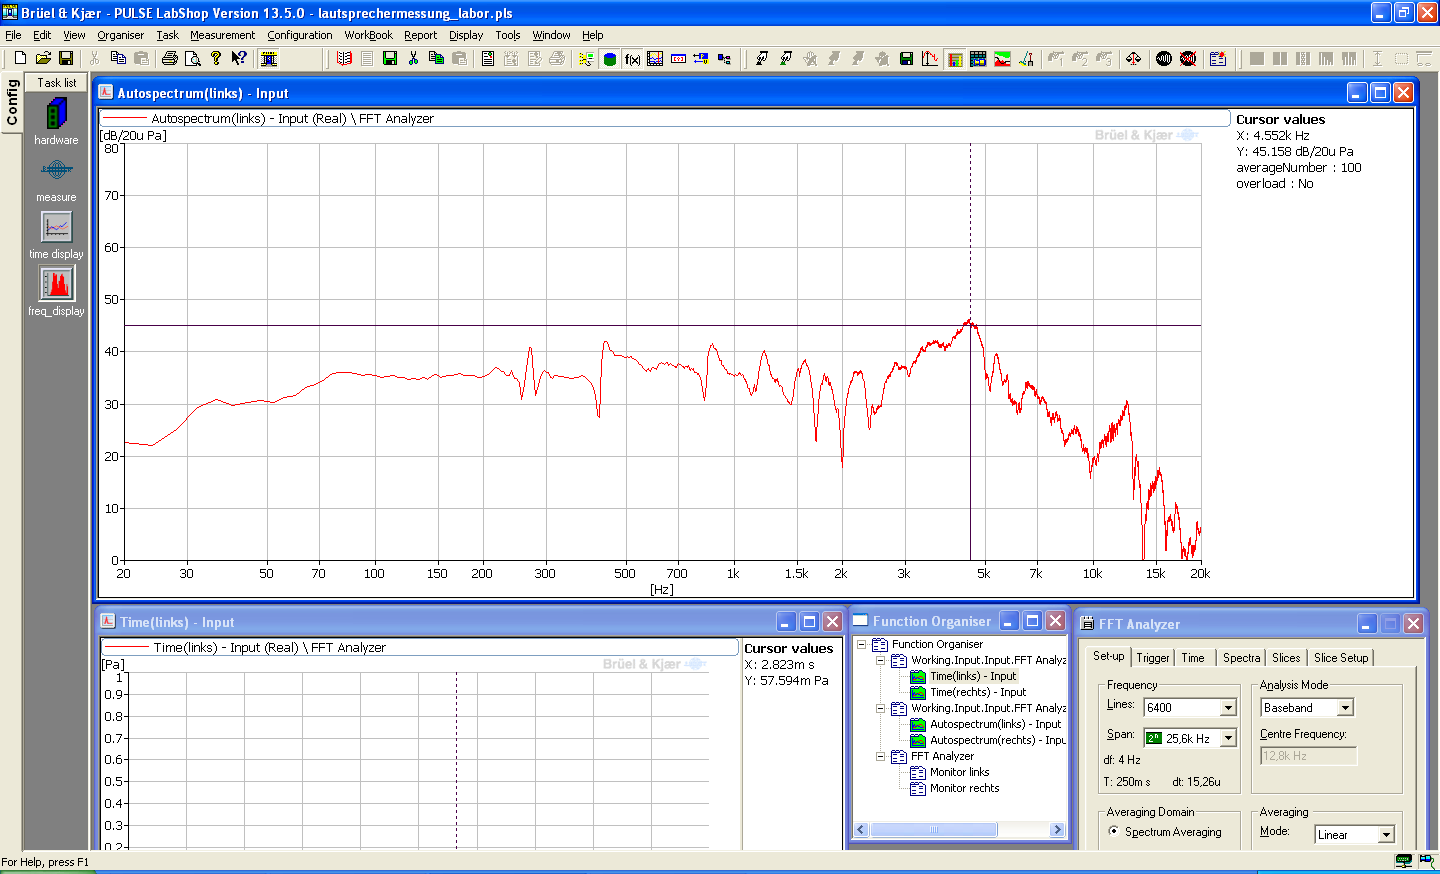
\includegraphics[width=0.7\textwidth]{img/LSMessung/TT/TT1mitSilikon.png}}\quad
	\subfloat{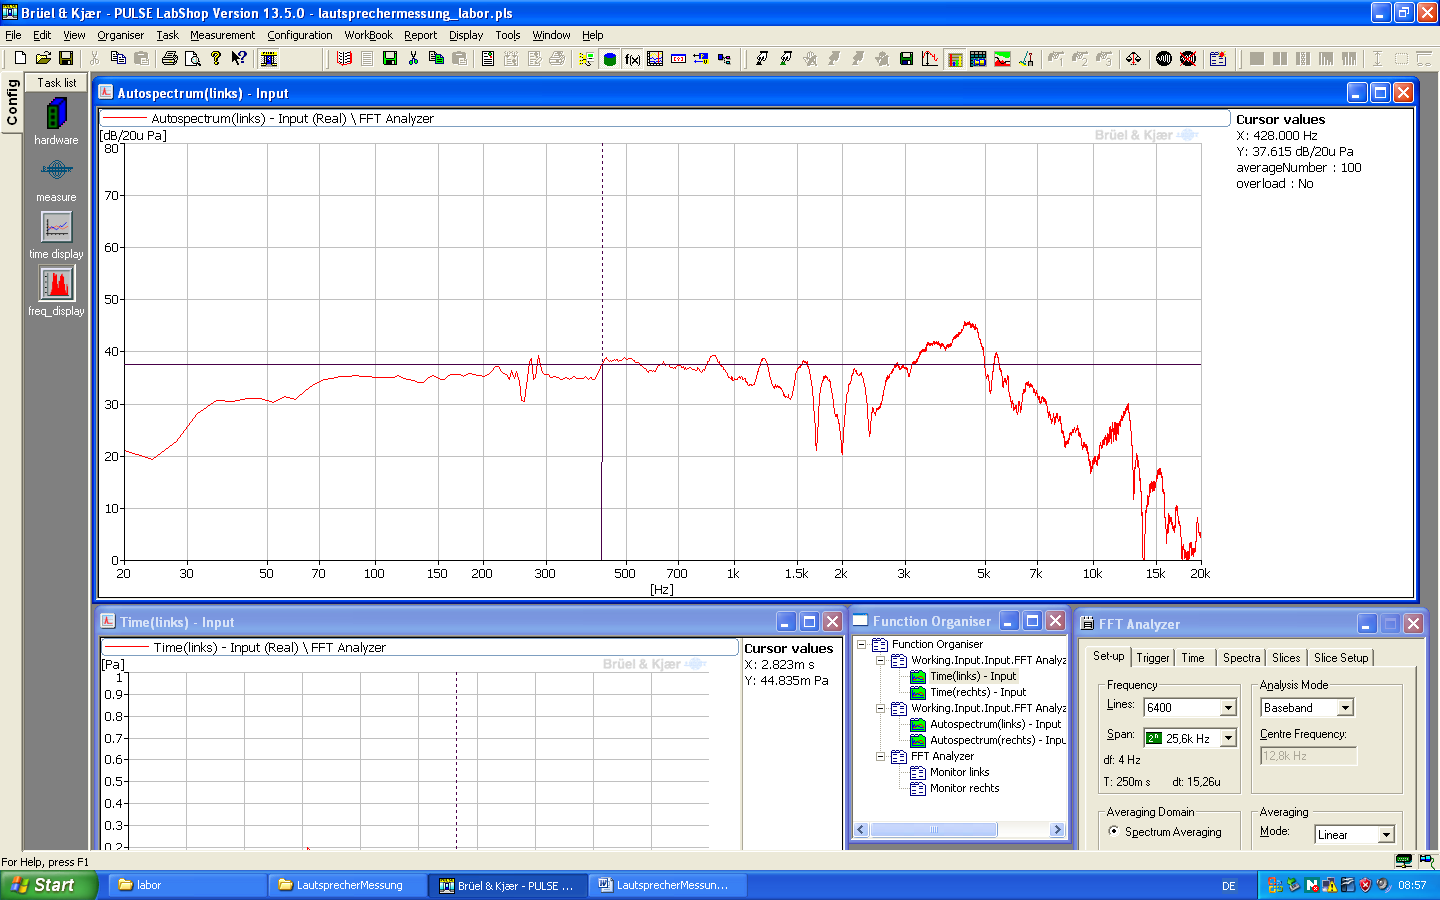
\includegraphics[width=0.7\textwidth]{img/LSMessung/TT/TT1mitSilikonUndWolle.png}}
	\caption{Tieftöner-Messung ohne Wolle\\ \enquote{TT1} (oben) und mit Wolle \enquote{TT1} (unten) | Boxenvolumen: 13,72l}
	\label{fig:5.3.4.1}
\end{figure}
Es ist die Verringerung der Welligkeit im Teiftonbereich (<1kHz) sichtbar.
In dieser Situation sollte der Tieftöner im besten Fall bis 1kHz spielen.
Des weiteren sollte er besser mit Wolle versehen werden.

\newpage
Als Referenz wird der Lautsprecher \enquote{TT2} gemessen. 
Ebenfalls einmal ohne und einmal mit Wolle im Gehäuse.
\begin{figure} [H]
	\centering
	\subfloat{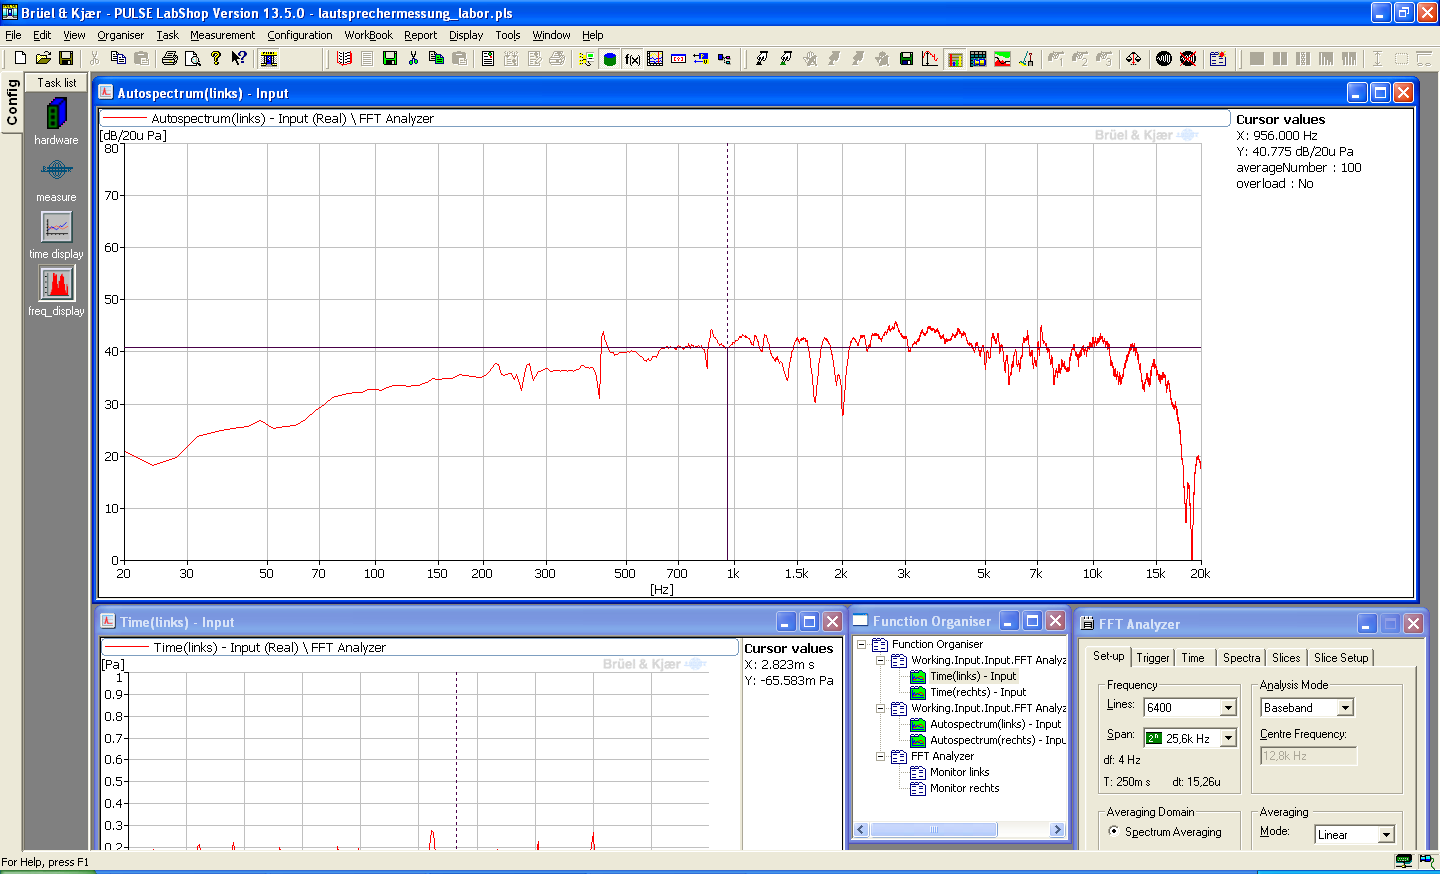
\includegraphics[width=0.7\textwidth]{img/LSMessung/TT/TT2mitSilikon_ohneWolle.png}}\quad
	\subfloat{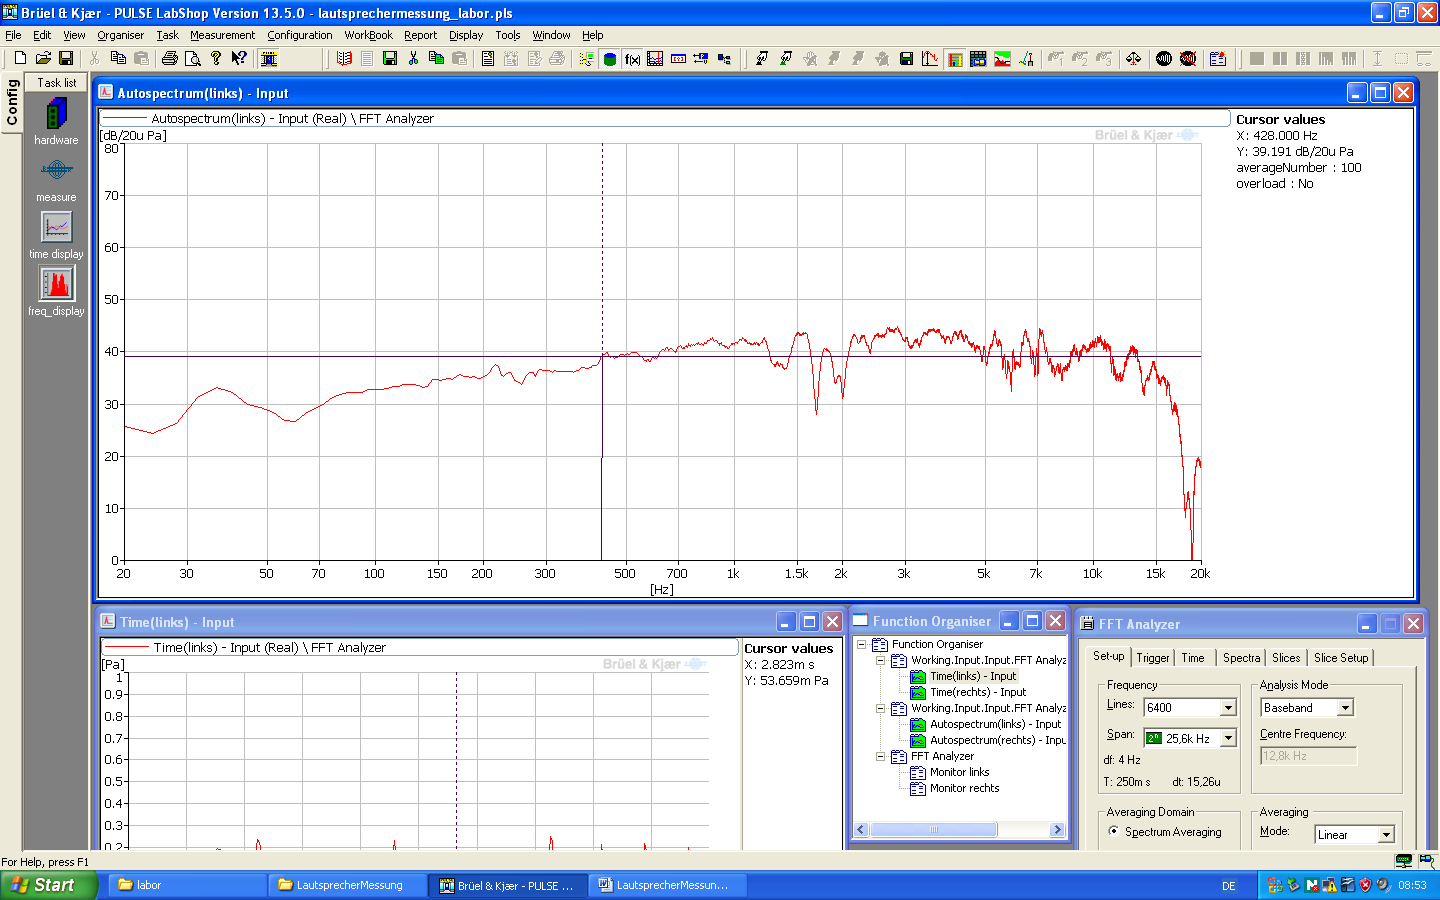
\includegraphics[width=0.7\textwidth]{img/LSMessung/TT/TT2mitSilikon_mitWolle.png}}
	\caption{Tieftöner-Messung ohne Wolle\\ \enquote{TT2} (oben) und mit Wolle \enquote{TT2} (unten) Boxenvolumen: 13,72l}
	\label{fig:5.3.4.2}
\end{figure}
Dieser Lautsprecher weist eine einigermaßen vertretbare Welligkeit im Mittel- und Hochton-Bereich auf.
Beim Niederton-Bereich ist der Schalldruckpegel jedoch geringer.
Der Mono-Subwoofer müsste bis einige 100-Hertz spielen um diese Schwäche auszumerzen.
Ein Subwoofer sollte jedoch nicht über 150 bis 200 Hz kommen, da Frequenzen unterhalb dieser Grenze nicht lokalisiert werden können.
Dieser Effekt ist für einen richtigen Subwoofer-Lautsprecher typisch.
Wieder ist ersichtlich, dass mit Wolle die Welligkeit im Mittel und Tiefton-Bereich etwas verringert wird.

\newpage
Durch ein paar weitere Messungen wurde der TT2 bereits sehr früh aus der Auswahl genommen und der Fokus auf den TT1 gelegt, da dieser im Tieftonbereich besser funktioniert.
\\
Außerhalb der Messungen für die Diplomarbeit wurde der Lautsprecher TT1 etwas beschädigt.
Die \enquote{Dustcap} des Lautsprechers wurde eingedrückt.
Für einen Tieftöner ist das nicht so schlimm, da die \enquote{Dustcap} in diesem Fall rein für den Schutz vor Staub zuständig ist.
Dies ist notwendig um den Bewegungsfreiraum zwischen der Spule an der beweglichen Membran und der Spule am fixierten Gehäuse gewährleisten zu können.
Wenn dieser Schutz nicht vorhanden ist, ist meist auch der Lautsprecher kaputt.\\
Bei einem Hochtöner wäre bereits das Eindrücken der Dustcap ein Todesurteil für den Lautsprecher, da die Kappenstruktur der Dustcap in diesem Frequenzbereich immensem Einfluss auf den Klang nimmt.
\\ \\
Nach Feststellen des Schadens wurde der Frequenzgang des TT1 erneut überprüft und er wies keine wesentlichen Veränderungen auf, was zu dem Schluss führte, dass er normal weiter gemessen wurde.\\
Als nächster Schritt werden die Tieftöner unter variierendem Volumen gemessen.
Dafür wird, wie zuvor erwähnt, hauptsächlich Ytong und Styropor verwendet.
Styropor gilt auch als einigermaßen schalltotes Material.
Da keine fixen Angaben gemacht wurden was die Schalldichte von Styropor betrifft, wurde eine Referenzmessung mit Ziegeln gemacht(Siehe Kapitel \ref{label}). % Referenzmessung Styropor, Ziegel einbauen!
\\
Das Volumen wird zuerst einmal stark verringert, um zu sehen ob überhaupt ein Effekt merkbar ist.
Dafür wird das Volumen von 13,72l auf 4,87l verringert.
\begin{figure} [H]
	\centering
	%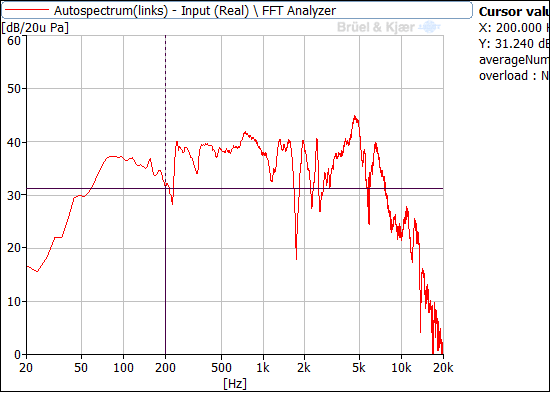
\includegraphics[width=0.75\textwidth]{img/LSMessung/TT/TT1silikon_4-87lVolumen.png}
	\caption{\enquote{TT1} | Boxenvolumen = 4,87l}
	\label {fig:5.3.4.3}
\end{figure}

%Vergleich mit original machen











